\documentclass[a4paper,12pt,dvipdfmx]{jreport}

\usepackage[dvipdfmx]{graphicx}
\usepackage{cite}
\usepackage{ascmac}
\usepackage{amsmath}
\usepackage{algorithm, algpseudocode}

%%% site-sty

%%% original
\usepackage{sty/NGC}
\title{2×3ミキサーを含む希釈木に対する\\NTMを実現するPMDへのマッピング法の適応}
\author{平井 将隆}
\stdnum{2600180248-7}
\date{20XX年度}


\begin{document}
\baselineskip 1.9zw
\maketitle


\newpage
\thispagestyle{empty}
\pagenumbering{roman}
\setcounter{page}{1}
\chapter*{内容梗概}
%\newcommand{\rout}[1]{\textcolor{red}{#1}}
%\newcommand{\bout}[1]{\textcolor{blue}{#1}}
%\newcommand{\gout}[1]{\textcolor{green}{#1}}
%\newcommand{\cout}[1]{\textcolor{cyan}{#1}}
%\newcommand{\mout}[1]{\textcolor{magenta}{#1}}
%\newcommand{\yout}[1]{\textcolor{yellow}{#1}} など色変可
ver2:ver1でalainさんに指摘された点について修正し,その部分を赤色にしました.
あと,第1章でのNTMという単語の説明・用法を,参考文献に忠実になるよう修正しました.

ver3:ver2で山下先生に指摘された点について修正し,その部分を青色にしました.
あと,「入力として受け取る」などまわりくどい表現をしてしまっていたのは,恐らくNTMの入出力関係を明記していなかったためなので,
NTMの名前が出た文の直後にその入出力関係についての文を青色で書きました.
フラッシングの説明も青色で書きました.

ver4:ver3で山下先生に指摘された点について修正し,その部分を緑色にしました.

ver5:第2章とver4で山下先生に指摘された点について修正したところを,シアン色にしました.

\newpage
\tableofcontents
\listoffigures
\listoftables

\newpage
\pagenumbering{arabic}
\chapter{はじめに}
\begin{itemize}
 % デフォルトの箇条書きは項目間や段落間のスペースが広いので下記のように調整した方が綺麗に見えるかも
 
 \setlength{\parskip}{0cm} % 段落間
 \setlength{\itemsep}{0cm} % 項目間
 \item どのような分野の研究か,その背景について説明する.
     \begin{itemize}
        \item 近年, 生化学分野において実験室規模で行われていた従来の実験に代わる新たな実験の装置としてバイオチップが注目されている.
        \item バイオチップの一種にPMD(Programmable Microfluidic Device)がある.
        \item PMDでは,バルブの開閉によってセル内の液滴を制御し,液滴の移動や混合を実現する.
    \end{itemize}
 \item その分野の従来の研究状況について説明する.
     \begin{itemize}
        \item PMDには,セル間での液滴の移動が原則的に不可能という欠点がある.したがって,その欠点を補い,セル間の移動無しで試薬の混合を行う試薬混合手法NTM(No Transport Mixing)が提案されている.
    \end{itemize}
 \item そして,何が解決すべき問題(本論文で扱った問題)かを説明.
     \begin{itemize}
        \item NTMを実現する既存の希釈木のPMDへの混合手順の決定法は,2×2ミキサーのみを含む希釈木にしか対応していない.したがって,入力として与えることができる希釈木の種類は限られている.
        {\item 2×3ミキサーを用いると,多くの子ミキサーを持つ場合がある.その場合,子ミキサーどうしのオーバーラップが発生しやすいため,ミキサーの配置が難しい.}
    \end{itemize}
 \item どのようなアイデアで解決したか,キーアイデアを少しだけ披露
     \begin{itemize}
         \item {希釈木が2×3ミキサーを含んでいた場合も液滴の移動無しでの混合手順を生成できるよう混合手順生成アルゴリズムに工夫を施した.
            \begin{itemize}
                    \item 入力希釈木に対して変形操作を行う.
                    \item PMD上へのミキサーの配置順を変更する.
            \end{itemize}}
    \end{itemize}
 \item どのような(実験)結果が得られたか、アピール(目次案の段階では希望的予測)
     \begin{itemize}
        \item 変形操作を行った後に入力希釈木をPMDへとマッピングすることにより,希釈木の変形を行わなかった場合と比較して,平均17\%のFlushing回数の減少が見られた.
     \end{itemize}

\item 章構成
    \begin{itemize}
    \item 第2章:PMDの概要,{2×2ミキサーを用いた液滴の移動の無い混合手順の生成}
    \item 第3章:{2×3ミキサーを用いた液滴の移動の無い混合手順の生成}
    \item 第4章:提案手法の評価方法とその結果
    \item 第5章:まとめと今後の課題
    \end{itemize}

\end{itemize}

\chapter{基礎知識}
本章では,本論文で扱うProgrammable Microfluidic Device(PMD)\mout{と呼ばれる}バイオチップの基礎知識について説明をする.
まず,PMDのアーキテクチャについて説明する.
\mout{その後},PMDのアーキテクチャの欠点についても説明する.
最後に,既存手法として,PMDのアーキテクチャの欠点に対応したPMD上での混合手順の生成手法
No Transport Mixing(NTM)について簡単に説明する.
\section{PMD}
\label{PMD}
本節では,PMDのアーキテクチャがどういった特徴や欠点を持つかを説明する.
\subsection{PMDのアーキテクチャ}
\label{arc}
%PMDとはどういうデバイスか説明を書く.
PMDの顕微鏡写真を図~\ref{fig:micrograph}に示\cout{す}~\cite{1}.
図~\ref{fig:micrograph}において,赤黒く見えるのはバルブと\mout{呼ばれる}部品で,バルブによって囲まれていて青い線の交点と重なっている領域はセルと呼ばれる.
バルブは開閉の操作を行うことが可能である.
図~\ref{fig:mixing}は,PMD上に流し込まれた2種類の試薬が混合される様子を\cout{示}している~\cite{4}.
図~\ref{fig:mixing}(a)から(b)は,圧力をかけられることで試薬が入力ポートからPMDの内部へと流し込まれる様子を\cout{示}している.
図~\ref{fig:mixing}(c)は,バルブの開閉の制御によって,ミキサーと呼ばれる,セルが円環状に繋げられた流路が生成される様子を\cout{示}している.
ミキサー内のバルブの開閉を行うことにより,ミキサー内の液滴の混合が行われる.
液滴の混合後は,図~\ref{fig:mixing}(d)で\cout{示}されているようにミキサー内のどのセルにおいても格納されている液滴の濃度は等しくなる.

また,PMDでは,図~\ref{fig:4and6Mixer}で\cout{示}したよう\mout{に}様々な大きさのミキサーを生成すること\mout{が}できる.
図~\ref{fig:4and6Mixer}(a)は2$\times2$のセルを用いる2$\times2$ミキサー,図~\ref{fig:4and6Mixer}(b)は2$\times$3セルを用いる2$\times$3ミキサーである.
\cout{PMDでは,}これら以外にも様々な大きさのミキサーの生成,及び,そのミキサー上での試薬の混合が可能である.
\begin{figure}[tbp]
 \centering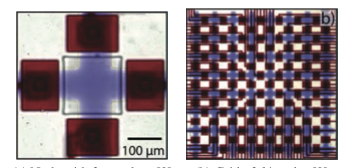
\includegraphics[scale=1.2]{img/PMDMicrograph.pdf}
 \caption{PMDの顕微鏡写真,参考文献~\cite{1}より引用}\label{fig:micrograph}
\end{figure}
\begin{figure}[tbp]
 \centering\includegraphics[scale=1.0]{img/PMDMixing_jp.pdf}
    \caption{PMD上に流し込まれた2種類の試薬が混合される様子,参考文献~\cite{4}より引用し一部改変}\label{fig:mixing}
\end{figure}
\begin{figure}[tbp]
    \centering\includegraphics[scale=0.5]{img/Modified_4and6Mixer.pdf}
 \caption{PMDで生成可能なミキサー}\label{fig:4and6Mixer}
\end{figure}
\newpage
\subsection{PMDにおけるセル間の液滴の移動}
%既存手法の説明への前提知識として,PMDにおいてセル間での液滴の移動操作は原則不可能であるということを説明する.
バイオチップの中心的なアーキテクチャであるDMFB(Digital Microfluid biochip)においては,PMDでのセルに相当する電極の間での液滴の移動操作~\cite{B110474H}を用い,試薬合成が行われる~\cite{5605330}\cite{10.1007/s11047-006-9032-6}\cite{10.1145/2429384.2429464}.
それに対して,PMDでは,セル間での液滴の移動操作は原則不可能であることが知られている.
図~\ref{fig:fluidseg}は\mout{,Flow-based Microfluidic Biochip(FMB)と呼ばれるバイオチップにおいて一般的に使用される液体の移動操作の手法を応用し,PMD上での試薬液滴の移動操作を試みたものの,失敗した際の様子を示している}~\cite{4}. 

\mout{この試薬液滴の移動操作の手法は,試薬液滴と油は混じり合わないという特性を利用し,油に試薬液滴を乗せた液体に圧力をかけることで試薬液滴を移動させる.
\mout{また,}移動経路上の届け先セルのところには油のみを通すマイクロ流体ラッチと呼ばれる特殊なバルブを備え付けておく.
これにより,届け先セル上に試薬液滴のみが濾し取られ,試薬液滴の移動操作が実行されるというものである.}
図~\ref{fig:fluidseg}(a)は,始点セルから届け先セルへの\cout{試薬}液滴の移動操作を試みる前の状態を\cout{示している.}
\mout{また,}図~\ref{fig:fluidseg}(b)は,油のみを通すマイクロ流体ラッチ~\cite{urbanski2006digital}と油を用いて始点セルから届け先セルへの試薬液滴の移動操作を試みた後の様子\cout{を示している}.
\mout{図~\ref{fig:fluidseg}(b)では,油に試薬液滴を載せた液体の移動経路上において試薬液滴の分割が発生している~\cite{FU2015343}.}
\mout{これは,油に試薬液滴を載せた液体の移動経路上の直角のところで\cout{試薬}液滴にかかる力が,部分ごとに均一でなくなるからである.}

以上で述べたように,経路上において液滴の分割が発生するため,PMDにおけるセル間の液滴の移動操作は不可能である.
したがって,PMDで試薬合成を行うためには,セル間での液滴移動のない混合手順を生成する必要がある.
\begin{figure}[tbp]
    \centering\includegraphics[scale=0.9]{img/FluidSegmentation.pdf}
 \caption{fluid segmentationの様子,参考文献~\cite{4}より引用し一部改変}\label{fig:fluidseg}
\end{figure}
\newpage
\section{{2×2ミキサーを用いた液滴移動の\bout{ない}混合手順の生成}}
%セル間の液滴の移動操作を必要としない試薬混合手法NTM(No Transport Mixing)の説明をする.
%その後,既存の希釈木のNTMでのPMDへのマッピング手法を説明する.
\ref{arc}~節で述べた通り,PMDで試薬合成を行うためには,セル間での液滴移動のない混合手順を生成する必要がある.
したがって,本節では既存のPMD上でのセル間の液滴移動のない混合手順の生成手法NTM(No Transport Mixing)の説明をする.
図~\ref{fig:ntmresult}はNTMの入出力データを\cout{示}している~\cite{4}.
NTMは,図~\ref{fig:ntmresult}(a)\cout{が示し}ているような希釈木を入力として受け取り,図~\ref{fig:ntmresult}(b)から(e)
\cout{が示し}ているような,希釈木に対応したPMD上での液滴の移動のない混合手順を生成する.
希釈木とは,試薬合成で目標濃度の\cout{混合}液滴を得るために,\cout{液滴の混合をどのように行えば良いか}を木で表したものである.
図~\ref{fig:ntmresult}(a)の希釈木において,ミキサーでの液滴の混合はM1からM4のミキサーノードで表され,
\mout{ミキサーでの液滴の混合で用いられる}試薬液滴は,\mout{希釈木の葉に位置する}試薬\mout{液滴}ノードで表されている.
また,図~\ref{fig:ntmresult}(a)の希釈木のエッジに付加された重みは,親ミキサーノードが\mout{子ミキサーノードや子試薬液滴ノード(子ノード)}から受け取る液滴の数を表している.

\ref{arc}~節で述べたように,PMDは2$\times$3ミキサーなど,2$\times$2以外の大きさを持つミキサーを生成できる.
しかし,本節で紹介してきたNTMには,2$\times$2ミキサーノードのみを含む希釈木しか扱うことができないという制約がある.
この制約のために,NTMが扱うことのできる希釈木の種類は大きく制限されている.
したがって,PMD上の液滴移動のない混合手順の生成手法には,NTMより多くの種類の希釈木を扱うことが出来るように拡張する余地がある.
NTMでは扱えなかった希釈木を扱えるようになれば,手法としての汎用性は高まる.
\begin{figure}[tbp]
 \centering\includegraphics[scale=0.7]{img/NTM.pdf}
    \caption{NTMの入力データと出力データ,参考文献~\cite{4}より引用し一部改変}\label{fig:ntmresult}
\end{figure}


\chapter{{2×3ミキサーを用いた液滴移動の\bout{ない}混合手順の生成}}
\label{proposed}
\section{アルゴリズムの概要}
\bout{本}章では,本論文の提案手法である2$\times$3ミキサーを用いた液滴移動の\mout{な}いPMD上での混合手順の生成手法の処理の流れを擬似コードを交えて説明する.


まず,本論文の提案手法の入出力について説明する.
本論文の提案手法の入力は,図~\ref{fig:inputoutput}(a)の,2$\times$2ミキサーノードと2$\times$3ミキサーノード,試薬液滴ノードの3種類のノード\mout{によって}構成されている希釈木である.
また,本論文の提案手法の出力は,図~\ref{fig:inputoutput}(b)から(e)の,入力希釈木に対応したPMD上でのミキサーの混合手順である.
図~\ref{fig:inputoutput}の(b)から(e)において,同じ図内のミキサーは,混合されるタイミング(タイムステップ)が同じミキサー同士である.

希釈木内のノードの,親ミキサーノード,子ミキサーノード,子試薬液滴ノードに対応\mout{する}ミキサーや試薬液滴のことを,親ミキサー,子ミキサー,子試薬液滴と呼ぶ.
図~\ref{fig:inputoutput}の(b)から(e)の混合手順において\mout{も,図~\ref{fig:ntmresult}の(b)から(e)のNTMが生成する混合手順と同様に},子試薬液滴や子ミキサーは,親ミキサーの配置されるセルに液滴を残\bout{さなければならない}.
親ミキサーは,それらの液滴を配置された場所で混合\mout{する}.

\begin{figure}[tbp]
 \centering 
    \includegraphics[scale=0.50]{img/OutPut.pdf}
 \caption{提案手法の入出力}\label{fig:inputoutput}
\end{figure}

\begin{algorithm}[tbp]
 \caption{提案手法の処理の流れ}\label{alg:all}
 \begin{algorithmic}[1]
     \Require $\mathit{Tree}$:2$\times$2ミキサーノードと2$\times$3ミキサーノード,試薬液滴ノードを含む希釈木 
     \Require $\mathit{PMDSize}$:使用するPMDのサイズ
     \State $\mathit{TransformedTree} \gets$ \Call{TransformTree}{$Tree$} \Comment{希釈木の変形操作}\label{transform_pseudo}
     \State $\mathit{MixInfo \gets}$\Call{GenMixOrder}{$\mathit{TransformedTree,PMDSize}$} \Comment{混合手順の生成} \label{xntm_pseudo}

      \Return $\mathit{MixInfo}$
 \end{algorithmic}
\end{algorithm}
Algorithm~\ref{alg:all}に本論文の提案手法のアルゴリズム全体の擬似コードを\mout{示す}.
本論文の提案手法は大きく分けると,Algorithm~\ref{alg:all}の\ref{transform_pseudo}行目の希釈木の変形操作と,\ref{xntm_pseudo}行目のPMD上での液滴の移動のない混合手順の生成の,2つの処理によって構成されている.

\section{入力希釈木の変形アルゴリズム}
まず,1つ目の処理である,Algorithm~\ref{alg:all}の\ref{transform_pseudo}行目の,希釈木の変形操作の説明を行う. 希釈木の変形操作は,希釈木を入力とし,変形された希釈木を出力する. 変形操作を高さ3の希釈木に対して行った場合の例を図~\ref{fig:Transform}に示\mout{す}.
図~\ref{fig:Transform}(a)は変形前の希釈木,図~\ref{fig:Transform}(b)は変形後の希釈木である.

\begin{figure}[tbp]
 \centering\includegraphics[scale=0.53]{img/Transform.pdf}
 \caption{希釈木の変形操作}\label{fig:Transform}
\end{figure}

希釈木の変形操作では,まず,希釈木内の各ノードに\bout{予測混雑度を割り当てる.本論文では,予測混雑度として各ミキサーノードをルートとする部分木内に含まれるミキサーノードの\rout{,それぞれのミキサーの大きさによって決まる評価値の和}を用いる.}
\bout{予測混雑度の割当後,}親ミキサーノードと,その全ての子ミキサーノードとの間に張られているエッジの順番を,各子ミキサーに割り当てられた予測混雑度をキー値にして降順でソートする. 
希釈木の変形操作のアルゴリズムの擬似コードは,Algorithm~\ref{alg:transform}に示す.

具体例を用いて,希釈木の変形操作で行われる処理を説明する.
%\rout{ミキサーノードM$_N$の予測混雑度の値をECV(M$_N$),M$_N$をルートとする部分木の予測混雑度を\rout{EvalMixer}(M$\mathit{_N}$)とする.}
\rout{ミキサーノードM$_N$の予測混雑度の値をECV(M$_N$)とする.}
\rout{図~\ref{fig:Transform}において,ECV(M$_1$) =  1.5*1.5*(1+ECV(M$_5$)) = 1.5*1.5*1 = 2.75,ECV(M$_2$) = 1.0*1.0*(1+ECV(M$_6$)) = 1.0*1.0*1 = 1.0,ECV(M$_3$) = 1.5*(1.0*(1+ECV(M$_7$))+1.5*(1+ECV(M$_8$))) = 1.5*(1.0+1.5) = 3.75,ECV(M$_4$) = 1.0 *(1.0*(1+ECV(M$_9$))+1.0*(1+ECV(M$_{10}$))) = 1.0*(1.0+1.0) = 2.0である.}
\rout{ECV(M$_3$) $>$ ECV(M$_1$) $>$ ECV(M$_4$) $>$ ECV(M$_2$)であるため,図~\ref{fig:Transform}での希釈木の変形においては,それぞれをルートとする部分木の位置が,予測混雑度で降順になるように並び替えられている.}
\begin{algorithm}[tbp]
 \caption{希釈木の変形操作}\label{alg:transform}
 \begin{algorithmic}[1]
     \Require $\mathit{Tree}$:2$\times$2ミキサーノードと2$\times$3ミキサーノード,試薬液滴ノードを含む希釈木 

     \Function {TransformTree}{$\mathit{\bout{Tree}}$}
        \State $\mathit{Children}$ = array()
        \ForAll {$\mathit{child}\gets \mathit{Tree.root.Children}$}
            \State $\mathit{\bout{ECV}}=$\rout{\Call{ ECV}{$child$} }\Comment{\rout{希釈木の部分木のルートである$\mathit{child}$の予測混雑度}}
            \State Children.append(($\mathit{\bout{ECV},child}$))
        \EndFor 
        \State $\mathit{SortedByECV} \gets $sorted($Children,reverse=$\True)\Comment{$\mathit{ECV}$をキー値に降順でソート}
        \State $\mathit{res}\gets$array()
        \ForAll {$\mathit{ECV,child}\gets \mathit{SortedByECV}$}
            \State $\mathit{SubTree}\gets $\Call {TransformTree}{$\mathit{child}$}
            \State $\mathit{res}$.append($\mathit{SubTree}$) \EndFor 
        \State \bout{$\mathit{TransformedTree}\gets \mathit{Tree}$ }
        \State \bout{$\mathit{TransformedTree.root.Children}\gets \mathit{res}$}\Return \bout{$\mathit{TransformedTree}$ }
    \EndFunction 
    
     \State \rout{$\mathit{MixerVal}\gets$array($-1,\mathit{Tree.MixerNum}$)}
     \Function {ECV}{$\mathit{\bout{Tree}}$}
        \If {\rout{$Tree.root.isMixer == False$}}\rout{\Return 0}
        \Else 
            \State \rout{$\mathit{idx}\gets \mathit{Tree.root.MixerIndex}$}
            \If {$\rout{\mathit{MixerVal[idx]} \geq 0}$}\Return \rout{MixerVal[idx]}
            \Else 
                \State \rout{ $\mathit{v}\gets 0$}
                        \State \rout{$\mathit{pweight} \gets 1.0$}
                        \If {\rout{$\mathit{Tree.root.size}== 6 $}}
                            \State \rout{$\mathit{pweight} \gets 1.5$}
                        \EndIf
                \ForAll {$\rout{\mathit{child}\gets \mathit{Tree.root.Children}}$}
                    \If {\rout{$\mathit{child.isMixer} $}}
                        \State \rout{$\mathit{weight} \gets 1.0$}
                        \If {\rout{$\mathit{child.size}== 6 $}}
                            \State \rout{$\mathit{weight} \gets 1.5$}
                        \EndIf 
                        \State \rout{$v+=\mathit{pweight*weight*(1+}$\Call{ECV}{$\mathit{child}$})}
                    \EndIf 
                \EndFor 
                \State \rout{$\mathit{MixerVal[idx]}\gets v$}
                \Return \rout{$\mathit{MixerVal[idx]}$}
            \EndIf
        \EndIf
    \EndFunction 
 \end{algorithmic}
\end{algorithm}
%次に,この変形操作の目的を説明する.

希釈木の変形操作とともに本論文の提案手法における中心的な処理である,PMD上での液滴の移動のない混合手順の生成では,親ミキサーの配置セルの一部が重なるよう,子ミキサーや子試薬液滴がPMD上に配置される.
この子ミキサーや子試薬液滴をPMD上へ配置する際に,その配置先のセルにはすでに試薬液滴やミキサー,中間液滴が配置されていることがある.この状態のことをオーバーラップと呼ぶ.

オーバーラップが発生した場合\rout{には},配置しようとしていたミキサーや試薬液滴のPMD上への配置の先延ばしを\rout{行うか},以降のタイムステップで混合に使われないPMD上の中間液滴を水で洗い流して,他の子ミキサーや子試薬液滴を配置するためのセルを空ける操作(フラッシング)\rout{を行う}.
フラッシングの回数が増えるほど,試薬合成で必要になる試薬量は増える.

\rout{高い予測混雑度を持つミキサーノードは,子孫ノードを多く持つ.}
したがって,高い予測混雑度を持つミキサーノードをルートとする部分木内のミキサーノードは,PMD上での配置先の近くに多くのミキサーや試薬液滴が配置されることになるため,オーバーラップ\bout{が発生する確率が高くなる.}
また,2$\times$2ミキサーノードは最大4個の子ノードを持つのに対して,2$\times$3ミキサーノードは最大6個の子ノードを持つ.
\rout{2$\times$3ミキサーノードを多く含む部分木は,2$\times$2ミキサーノードを多く含む部分木よりも,高い予測混雑度を持ちやすく,オーバーラップ\bout{が発生する確率が高くなる.}}

希釈木の変形操作は,\bout{PMD上へのミキサーや試薬液滴の配置が幅優先的に行われることを利用して,オーバーラップを減らせる可能性を高める.}
混合手順の生成処理では,希釈木のルートのミキサーノードから\mout{幅優先探索(BFS)の順番}で,各ノードに対応したミキサーや試薬液滴のPMD上での配置先を決めていく.
予測混雑度をキー値にし\mout{て}降順でソートを行えば,予測混雑度が高いミキサーノードほど,\mout{BFSの順番}において早くPMD上での配置先の決定を行う\mout{ようにな}る.
この仕組みにより,予測混雑度の高いミキサーノードほど,PMD上に空いたセルが多く,配置方法の自由度が高い\mout{タイムステップが小さいときに}配置が行える.
\mout{また,}オーバーラップを起こしやすい,配置優先度の高い部分木内のミキサーも,\mout{親ミキサーの配置先周辺に空いたセルが多く,配置方法の自由度が高いとき}に配置が行えるようになり,オーバーラップが起こりにくくなる.
オーバーラップが起こりにくくなれば,フラッシングの回数\mout{を}減らすことができる.





\section{\mout{PMD上での液滴移動のない混合手順の生成アルゴリズム}}
次に,2つ目の処理である,Algorithm~\ref{alg:all}の\ref{xntm_pseudo}行目の,PMD上での液滴移動のない混合手順の生成の説明を行う.
\mout{この処理は,}\mout{希釈木(図~\ref{fig:Transform}(b))}と,使用するPMDのサイズ\mout{(7$\times$7)}を入力とし,PMD上での液滴移動のない混合手順\mout{(図~\ref{fig:result}(a)から(e))}を出力する.
図~\ref{fig:result}(a)から(e)のPMDのセル\rout{上}に配置された\rout{数字$n$は$n$番目の試薬(R$_n$)の液滴を},PMDのセル\rout{外}に配置された\rout{数字$n$は$n$番目のミキサー(M$_n$)を}\rout{示す}.
図~\ref{fig:result}(a)から(e)の左下に書かれたTは混合が実行されるタイムステップ,Fはそのタイムステップに至るまでに行われたフラッシングの回数を\rout{示す}.

\begin{figure}[tbp]
 \centering\includegraphics[scale=0.6]{img/result.pdf}
    \caption{図~\ref{fig:Transform}(b)の希釈木を入力とした,PMD上での液滴移動のない混合手順の生成結果}\label{fig:result}
\end{figure}

\bout{図~\ref{fig:result}の混合手順の意味を説明する.}
\bout{図~\ref{fig:result}(a)は,タイムステップ1ではM$_5$,M$_7$,M$_9$での液滴の混合が行われることが表している.}
\bout{その後,図~\ref{fig:result}(a),(b)間でのFの増加は,フラッシングが行われ\rout{,}以降のタイムステップの\rout{,}ミキサーでの液滴の混合で用いられない中間液滴は水で洗い流されることを表している.}
\bout{図~\ref{fig:result}(b)は,タイムステップ2ではM$_1$,M$_6$,M$_8$,M$_{10}$での液滴の混合が行われるということ\rout{を示}している.}
\bout{以降の混合手順の図においても,各ミキサーでの液滴の混合と,フラッシングを行うタイムステップ\rout{を示している}.}


PMD上での液滴移動のない混合手順の生成過程で行われる処理は,主に以下に示した3つである.
混合手順の生成アルゴリズムにおいて,基本となる処理は処理~\ref{place}(配置)と処理~\ref{mix}(混合)である.
混合手順の生成アルゴリズムは,処理~\ref{place}(配置)と処理~\ref{mix}(混合)を繰り返す.
\bout{オーバーラップが発生し,}処理~\ref{place}(配置)と処理~\ref{mix}(混合)が行えなくなったら,処理~\ref{flush}(フラッシング)を行う.
その後,再び処理~\ref{place}(配置)と処理~\ref{mix}(混合)を行う.
これらの処理の繰り返し\mout{が},ルートのミキサーであるM$_0$の混合が行われるまで続け\mout{られ}る.
\bout{Algorithum~\ref{alg:genMixOrder}に\mout{PMD上での}液滴移動のない混合手順の生成アルゴリズムの擬似コードを示\mout{す}.}

\begin{itembox}[l]{混合手順を生成する過程で行われる処理}
\begin{enumerate}
    \item 配置(PMD上に配置されているミキサーの,子ミキサーや子試薬液滴のPMD上への配置)\label{place}
    \item 混合(PMD上に配置されているミキサーでの,液滴の混合)\label{mix}
    \item フラッシング(フラッシングによる,PMD上の空いたセルの確保)\label{flush}
    %\item 延期された配置(手順~\ref{place}で配置できなかったミキサーや子試薬液滴のPMD上への配置)\label{skipped}
\end{enumerate}
\end{itembox}


\begin{algorithm}[tbp]
 \caption{液滴移動のないPMD上での混合手順の生成アルゴリズムの擬似コード}\label{alg:genMixOrder}
 \begin{algorithmic}[1]
     \Require $\mathit{Tree}$:2$\times$2ミキサーノードと2$\times$3ミキサーノード,試薬液滴ノードを含む希釈木 
     \Require $\mathit{PMDSize}$:使用するPMDのサイズ
     \Function{GenMixOrder}{$\mathit{TransformedTree,PMDSize}$} 
     \State $\mathit{TransformedTree} \gets$\Call{TransformTree}{$\mathit{Tree}$} \Comment{希釈木の変形} 
     \State $\mathit{PMD}\,\gets $  PMDInit($\mathit{PMDSize}$)
     \State $\mathit{PMD}\,\gets $  PlaceOnPMD($\mathit{TransformedTree.RootMixer,PMD}$)
     \State $\mathit{ret} \gets $array() \Comment{混合手順を記録するための配列}

    \State \While{$TransformedTree.RootMixer.state \neq Mixed $ }
        \ForAll{$\mathit{mixer} \gets \mathit{PMD.MixerOnPMD}$} 
        \State $\mathit{AllChildrenPlaced}\gets\mathit{True}$
        \State $\mathit{AllChildrenMixerMixed}\gets\mathit{True}$
        \State $\mathit{ShouldFlush}\gets\mathit{True}$
        \ForAll{$\mathit{child} \gets \mathit{mixer.Children}$} 
            \If {$\mathit{child}\:\mathit{\mathbf{not}}\,\mathit{\mathbf{in}}\:\mathit{PMD.OnPMD}\:and\:$CanPlace($\mathit{child,PMD}$)}
                \State$\mathit{AllChildrenPlaced \gets False}$
                \State $\mathit{PMD}\, \gets$  PlaceOnPMD($\mathit{child,PMD}$) \Comment{子ミキサー,子試薬液滴の配置}
                \State $\mathit{ShouldFlush}\gets\mathit{False}$
            \EndIf 
            \If {$\mathit{child.kind}==\mathit{Mixer} \: \mathit{\mathbf{and}}\: \mathit{child.state}\neq\mathit{Mixed}$}
                \State $\mathit{AllChildrenMixerMixed}\gets\mathit{False}$
            \EndIf 
        \EndFor 
         \If{$\mathit{AllChildrenPlaced}\,\mathit{\mathbf{and}}\, \mathit{AllChildrenMixerMixed}$}
            \State$\mathit{PMD}\gets$Mix($\mathit{mixer,PMD}$)\Comment{ミキサーの混合}
            \State$\mathit{mixer.state} \gets \mathit{Mixed}$ 
            \State$\mathit{ret} $.append($\mathit{mixer}$) 
            \State $\mathit{ShouldFlush}\gets\mathit{False}$
        \EndIf
        \EndFor 
     \If{$\mathit{\rout{ShouldFlush}}$}
                    \State $\mathit{PMD}\gets$Flush($\mathit{PMD}$)\Comment{フラッシング}
                \EndIf
    \EndWhile 

     \Return $\mathit{ret}$
     \EndFunction
 \end{algorithmic}
\end{algorithm}


図~\ref{fig:process}は,図~\ref{fig:Transform}(b)の希釈木を入力として,7$\times$7サイズのPMD上で図~\ref{fig:result}の液滴移動のない混合手順を生成する過程を表している.
混合手順の生成は,図~\ref{fig:process}(a)のようにPMD中央部にルートのミキサー(M$_0$)を配置して開始される(処理~\ref{place}).
その後,図~\ref{fig:process}(b),(c)のように,子ミキサーや子試薬液滴が親ミキサーと一部のセルを共有するように,PMD上に配置される(処理~\ref{place}).
この際,オーバラップしている子ミキサーや子試薬液滴は配置を先延ばし\mout{される}. 配置を先延ばししたミキサーや試薬液滴以外の全てのミキサーや試薬液滴を配置し終えると,図~\ref{fig:process}(d)のように,ミキサー\bout{での液滴の}混合を行う(処理~\ref{mix}).
処理~\ref{place},処理~\ref{mix}\mout{を}それ以上行\mout{うことができなくなれば},図~\ref{fig:process}(e)のように,処理~\ref{flush}のフラッシングと,配置を先延ばしされていた試薬液滴やミキサーの配置(M$_2$,M$_8$,M$_{10}$)を行う(処理~\ref{place}).
図~\ref{fig:process}(f)では,M$_2$上に子ミキサーのM$_6$を,M$_8$とM$_{10}$に子試薬(R$_1$,R$_2$,R$_3$,R$_4$)を配置する(処理~\ref{place}).
\bout{これ以降の図で示されている混合手順を生成する過程においても,処理1,処理2,処理3の連続する処理を繰り返し行っている.}
図~\ref{fig:process}(j)では,ルートのミキサーであるM$_0$での液滴の混合(処理~\ref{mix}) を行\mout{い},試薬合成\mout{が完了\bout{する}}.

ミキサーでの試薬の混合を行っている,図~\ref{fig:process}(d),(g),(h),(i),(j)が,本論文の提案手法の出力,2$\times$3ミキサーを用いたPMD上での液滴移動のない混合手順である. \begin{figure}[tbp]
 \centering\includegraphics[scale=0.93]{img/process.pdf}
 \caption{液滴移動のない混合手順の生成過程}\label{fig:process}
\end{figure}


%\section{ライブラリを用いたモジュールの配置{アルゴリズム}}

%ライブラリを用いたモジュールの配置方法を例,図や擬似コードを用いながら説明する.


%希釈木の変形操作の手順や目的などを例や擬似コードを用いながら説明する.


\chapter{実験結果と考察}

\section{評価方法}
%入力希釈木の変形操作を用いた場合と用いなかった場合での希釈木のマッピング結果を比較して,
%入力希釈木の変形操作のFlushing操作を減少させる効果を評価する.
提案手法における希釈木の変形操作の評価を行うため,変形操作を行った希釈木と変形操作を行わなかった希釈木のそれぞれを入力として,
PMD上での液滴移動のない混合手順の生成を行う.
その後,それぞれの希釈木を入力として生成された混合手順において,必要になったフラッシングの回数を比較することで,
希釈木の変形操作によるフラッシングの回数の削減率を求め,希釈木の変形操作の有効性を測る.

具体的な評価方法を述べる.
まず,\rout{高さ}3,4,5の希釈木を,500個ずつランダムに生成する.
%その後,それぞれの高さごとの,すべての希釈木に関して,変形操作を行う希釈木と変形操作を行わない希釈木のそれぞれを入力とし,
\rout{その次に,}生成したすべての希釈木\rout{を入力とし},PMD上での液滴移動のない混合手順の生成を行う.
\rout{その後,生成したすべての希釈木に対して変形操作を行う.これらの変形を行った希釈木を入力として,PMD上での液滴移動のない混合手順の生成を行う.}
得られた混合手順の内,
%変形操作を行った希釈木と変形操作を行わなかった希釈木の,どちらを入力として生成された混合手順も
変形操作を行った\rout{希釈木と変形操作を行わなかった希釈木の,どちらの希釈木を}入力として生成された混合手順\rout{においても,}
必要になるフラッシングの回数が1以上だった場合のみ,\rout{その}希釈木\rout{における}変形操作によるフラッシングの回数の削減率を求める.
最後に,\rout{希釈木の高さごとの}削減率の平均(平均削減率)を求める.
平均削減率の値より,希釈木の変形操作の,混合手順で必要になるフラッシング回数の削減に対する有効性を測る.

\section{実験結果と考察}
%実験結果を表で載せる.実験結果から分かることや考察を述べる. 
表~\ref{table:result}に実験結果を示す.
また,図~\ref{fig:graph}には3,4,5の各高さの希釈木における,希釈木の変形操作によるフラッシングの回数の削減率を折れ線グラフで示す.

まずは,実験結果から分かることを述べる.
図~\ref{fig:graph}より,希釈木の高さが3,4,5と大きくなるにつれて,希釈木の変形操作によるフラッシングの回数の削減率は高くなっていることが分かる.
\rout{また,希釈木の}高さが最も小さい3\rout{の場合のみ},フラッシングの回数の平均削減率は負の値をとっており,希釈木の変形操作によってフラッシングの回数が増加していることが分かる.

%希釈木の高さが3のときの希釈木の変形によるフラッシングの回数の平均削減率が負になっていることと,変形操作の対象になる希釈木の高さが大きくなるほど,フラッシングの回数の平均削減率が高まっていることから,

次に,以上で述べた実験結果に対する考察を述べる.
高さの大きい希釈木になるほど,その希釈木における深さの小さい位置にあるミキサーノードは,多くの子孫ミキサーノードを持ち,割り当てられる予測混雑度の値が大きくなる可能性が高い.
これにより,高さの大きい希釈木における,深さの小さい位置にあるミキサーノード間でも,割り当てられる予測混雑度の値の差は大きくなる可能性が高く,予測混雑度の差が\rout{極端に小さい}場合での位置の入れ替えは少なくなる.
したがって,高さの大きい希釈木における,深さの小さい位置にあるミキサーノードに対する,オーバーラップの\gout{発生させ}やすさの評価指標として予測混雑度が上手くはたらき,フラッシングの回数の削減につながったと考えられる.
また,これに対して,高さの小さい希釈木においては,深さの小さい位置にあるミキサーノードに対しても,予測混雑度がオーバーラップの\gout{発生させ}やすさの評価指標として上手くはたらきにくく,フラッシングの回数の削減につながりにくいと考えられる.
\gout{この条件に沿う希釈木の例として,図~\ref{fig:h3}に示した希釈木がある.図~\ref{fig:h3}の希釈木に関する実験データは表~\ref{table:h3}に示した.}

表~\ref{table:result}から分かるように,希釈木の高さが大きいほど,希釈木内に含まれる2$\times$2ミキサーや2$\times$3ミキサーの平均個数は多くなる.
\rout{また,PMD上へのミキサーの配置の回数が増えるほど,オーバーラップの発生回数とフラッシングが必要になる回数は増える.}
\rout{したがって,希釈木の高さが大きいほど,その希釈木を入力として生成された混合手順内で必要になるフラッシングの絶対数は増加し,その削減が容易になる.}
\rout{以上の理由で,希釈木の高さが大きいほど,}フラッシングの回数の平均削減率が高くなったと考えられる.
また,これに対して,希釈木の高さが小さい場合は,その希釈木を入力として生成された混合手順内で必要になるフラッシングの\rout{回数の絶対数が少ないため,フラッシングの回数の}削減は難しいと考えられる.


以上の理由から,
現在の希釈木の変形操作の手法で有効な変形を行うためには,高さの大きい希釈木を扱う必要があると考える.
\rout{高さの低い希釈木内のミキサーノードの,オーバーラップの\gout{発生させ}やすさの評価指標として,予測混雑度が上手くはたらきにくい点に関しては,}
変形操作を施す希釈木の高さに応じて予測混雑度の計算方法を変更することで,対策を取ることができると考える.

\begin{table}[tbp]
\centering
\caption{実験結果(小数点2桁まで)}
\begin{tabular}{l|r|r|r|r|r|r|r} \Hline
    \multicolumn{1}{l|}{\multirow{2}{*}{希釈木の高さ}}& \multicolumn{2}{c|}{平均ミキサー数} &\multicolumn{2}{c|}{平均オーバーラップ数} &  \multicolumn{2}{l|}{平均フラッシング数} & \multicolumn{1}{l}{\multirow{2}{*}{\begin{tabular}{c}フラッシングの\\平均削減率($\%$)\end{tabular}}} \\\cline{2-7}
        &2$\times$2&2$\times$3&変形前&変形後&変形前&変形後&\\\hline\hline 
    %\multirow{2}{*}{希釈木の高さ}& \multicolumn{2}{c|}{\begin{tabular}{r|r}\multicolumn{2}{c}{平均オーバーラップ数}\\\cline{1-2}\end{tabular}} &  \multicolumn{2}{l|}{\begin{tabular}{c}変形ありでの\\平均フラッシング数\end{tabular}} & \multicolumn{1}{l}{\begin{tabular}{c}フラッシングの\\平均削減率($\%$)\end{tabular}} \\\hline\hline 
    3  &3.30&4.21& 2.64&2.66&1.78 & 1.79 & -2.30 \\\hline
    4  &7.03&9.29& 7.91&7.68&6.15&5.80&2.94  \\\hline
    5  &13.88&18.25& 17.64&16.92&14.35&13.39&4.96  \\\hline
\end{tabular}
\label{table:result}
\end{table}

\begin{figure}[tbp]
 \centering 
    %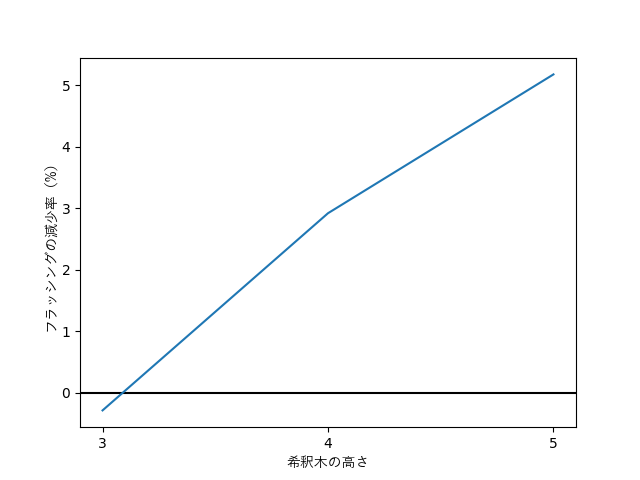
\includegraphics[scale=1.0]{img/decreasement.png}
    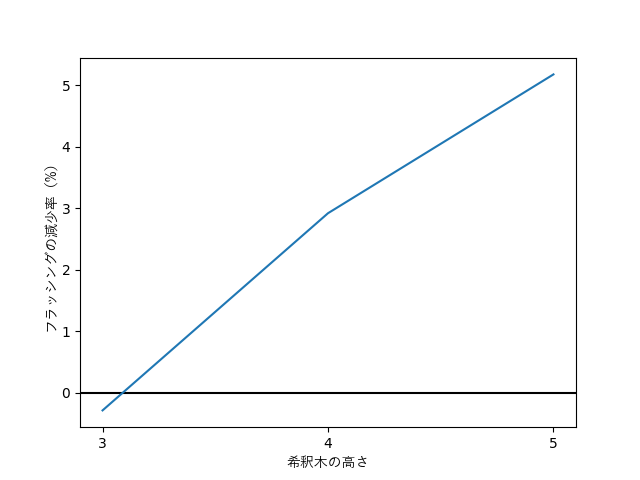
\includegraphics[scale=0.8]{img/decreasement.png}
 \caption{3,4,5のそれぞれの高さを持つ希釈木の,変形操作によるフラッシングの回数の平均削減率}\label{fig:graph}
\end{figure}

\begin{figure}[tbp]
 \centering 
    \includegraphics[scale=0.65]{img/h3.pdf}
 \caption{高さ3で,変形操作によってフラッシングの回数が増加する希釈木の変形}\label{fig:h3}
\end{figure}

\begin{table}[tbp]
\centering
    \caption{図~\ref{fig:h3}(a),(b)の希釈木から得られる混合手順内で発生するオーバーラップ数と,必要になるフラッシング数}
\begin{tabular}{l|r|r} \Hline
    &\multicolumn{1}{l|}{変形前の希釈木(図~\ref{fig:h3}(a))}& \multicolumn{1}{l}{変形後の希釈木(図~\ref{fig:h3}(b))}  \\\hline\hline
オーバーラップ数  & 4 & 5  \\\hline
フラッシング数  & 2&4  \\\hline
\end{tabular}
\label{table:h3}
\end{table}

\chapter{おわりに}
%\begin{itemize}
%\item 本論文の概要と特徴
%\item 得られた成果
%\item それから得られる最終結論
%\item 残された課題
%\end{itemize}
%を書く.
バイオチップの一種であるPMDは,バルブで囲まれたセルという領域が格子状に並んだ構造を持つ.
PMDでは,ミキサーと呼ばれる環状の流路で液滴の混合を行う.
また,PMDでは,セル間の液滴の移動は原則不可能である.
この特徴への対策として,PMD上で試薬合成を行う際は,セル間の液滴移動のない混合手順を取る必要がある.
しかし,既存のセル間の液滴移動のない混合手順生成手法(NTM)の扱うことができる入力データ(希釈木)の種類は,2$\times$2ミキサーノードのみを含む希釈木と,かなり限定されてい\gout{る}.
したがって,本論文では2$\times$2ミキサーのみでなく,2$\times$3ミキサーも用いたPMD上での液滴移動のない混合手順の生成手法を提案した.

2$\times$3ミキサーを扱うにあたって,PMD上でミキサー同士の配置セルが重なった状態(オーバーラップ)の発生や,オーバーラップへの対処(フラッシング)を行う
回数の増加を抑える必要がある.
本論文では,このオーバーラップやフラッシングの回数の増加への対処として,予測混雑度と呼ばれるミキサーノードの評価値を用いて希釈木へ変形操作を行う手法を提案した.

実験では,複数の高さの希釈木から,変形操作を行った場合と行わなかった場合の2つの希釈木を生成した.
そして,それぞれの希釈木をPMD上での液滴移動のない混合手順の生成手法の入力として与え,
その出力の混合手順内で必要になるフラッシングの回数を比較した.
この比較の結果として,希釈木の変形操作を行うことによる,混合手順内で必要になるフラッシングの回数の平均削減率が算出された.

平均削減率の値より,希釈木の高さが大きいほど,変形操作による混合手順内で必要になるフラッシング数の削減効果は高くなることが分かった.
また,高さの小さい希釈木に対する変形操作での,混合手順内で必要になるフラッシング数の削減効果は低いことも分かった.

最後に,残された課題を述べる.
高さの小さい希釈木に対する変形操作での,混合手順内で必要になるフラッシング数の削減効果を高めるためには,
予測混雑度の算出方法の変更が必要であると考えられる.
したがって,
高さの小さい希釈木に対する変形操作においても高いフラッシング数の削減効果を得られるような,予測混雑度の算出法を求めることは今後の課題である.
また,本論文内では詳しくは書いていないが,ミキサーのPMD上での配置先セルの決定は現在ヒューリスティックで行っている.
配置先セルの決定を行うヒューリスティックの改良を行えば,さらなるフラッシング数の削減を行える可能性もある.
したがって,このヒューリスティックの改良も今後の課題である.



\chapter*{謝辞}
本論文の執筆にあたり,研究内容や論文の書き方など手厚くご指導してくださった山下先生に感謝します.
また,論文執筆にあたり,拙い文章にもめげずに同期チェックをしていただいた有村優斗君,ありがとうございました.
最後に,大学に行き勉学に励む環境を与えてくださった家族に感謝します.


\bibliographystyle{junsrt}
\bibliography{ref}
\end{document}
